\fancyhead[LO, RE] {Studio delle Tecnologie}
\section{Studio delle Tecnologie}
\subsection{Stealth 3000}
La maggior parte delle aziende tessili di larga scala in Italia utilizza un ERP specifico, Stealth 3000, sviluppato dall'azienda italiana Dedagroup.\\
In quanto ERP connette tutti gli applicativi utilizzati dall'azienda, oltre ad essere un gestionale disegnato specificatamente per il mercato della moda. \\
Si tratta di un'applet Java, accessibile solo internamente all'azienda da Internet Explorer e Firefox.\\
Di seguito verrà illustrato il funzionamento di Stealth 3000 negli ambiti che sono stati toccati dal progetto CRM, che sono solo una minima parte di quanto offerto dall'ERP. Gli ambiti in questione sono i Soggetti, ovvero i clienti in generale, e le loro condizioni commerciali, gli oggetti e le loro classificazioni, ovvero gli articoli che vengono venduti ed infine i listini di vendita.\\
Tutti i contenuti anagrafici dei dati rappresentati sono fittizi, ottenuti dai manuali d'uso a scopo formativo.

\subsubsection{Soggetto}
Sono una qualunque entità fisica, giuridica, gestionale, organizzativa con cui l'azienda intrattiene rapporti di business.\\
Esempi di Soggetti sono: Clienti, Fornitori, Agenti,Terzisti, Importatori, Distribution Centers, Reparti interni.\\
L'archivio dei soggetti ne contiene i dati anagrafici fissi nel tempo (Ragione Sociale, Partita IVA, Indirizzo, ecc). Il soggetto ha una lista di indirizzi associati che ne definiscono punti di riferimento, ad esempio potrebbe avere un indirizzo di fatturazione ed un indirizzo di spedizione diversi tra loro.\\
Il soggetto può avere contemporaneamente più \textbf{Ruoli}; Esso rappresenta il tipo di rapporto che il Soggetto ha con l'Azienda, e può essere di tre tipi: \textbf{Cliente}, \textbf{Fornitore} o \textbf{Agente}. A seconda del ruolo ci sono differenti \textbf{Condizioni Commerciali}.
Di seguito la form di anagrafica Soggetto vista da Stealth 3000:
\newpage
\begin{figure}[!h]
\thispagestyle{empty}
\centering
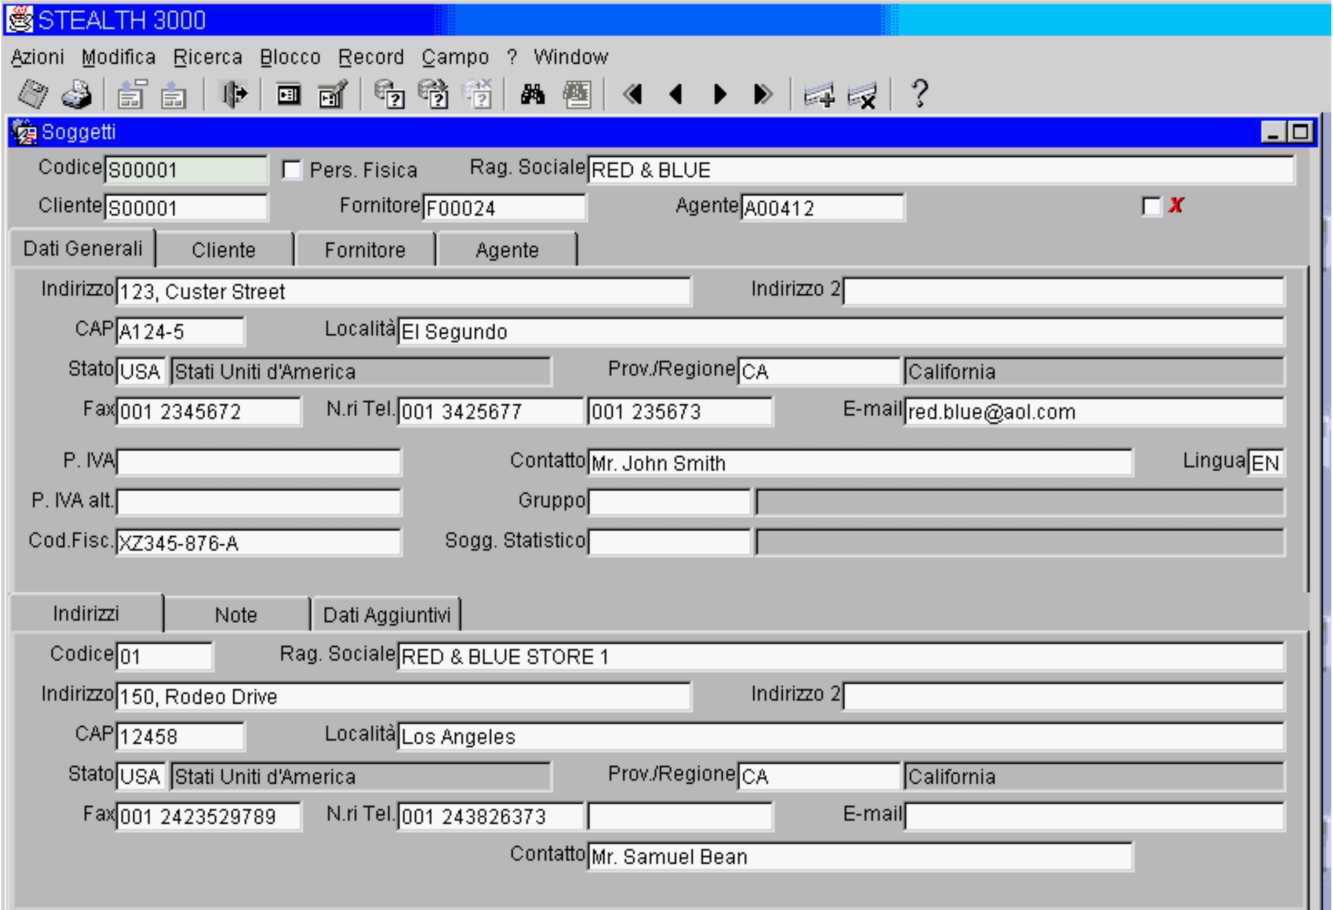
\includegraphics[scale=0.45]{img/SogAnag.png}
\caption{Anagrafica Soggetti}
\end{figure}
\newpage
Dati di testata:
\begin{table}[!h]
	\begin{center}
	
	\begin{tabular}{| c | c |}
	\hline
	\textbf{Dato} & \textbf{Descrizione} \\ \hline
	Codice & \begin{tabular}{@{}c@{}@{}@{}@{}@{}}  Codice Soggetto: in fase di creazione il codice\\ viene attribuito automaticamente all’uscita\\ del campo da un numeratore pubblico \\ma può essere forzato dall’utente.\\ Il sistema effettuerà in automatico un controllo\\ di unicità del codice all’interno del database.\end{tabular} \\ \hline

	Persona Fisica &  \begin{tabular}{@{}c@{}@{}@{}}   Flag che indica che il soggetto è una persona fisica\\ anzichè giuridica, per cui il campo della\\ Ragione sociale dovrà essere sostituito\\ dall’inserimento di Cognome e Nome.\end{tabular}\\ \hline

	Ragione Sociale & Descrizione della missione aziendale.\\ \hline
	
	Cliente &  \begin{tabular}{@{}c@{}@{}@{}@{}}  Codice corrispondente al ruolo cliente (se esistente)\\  del soggetto. Il codice sarà assegnato\\  in automatico alla generazione del ruolo\\ ed il campo presente servirà per ricerche \\mirate ai soli ruoli cliente.\end{tabular}\\ \hline
Fornitore &  \begin{tabular}{@{}c@{}@{}@{}@{}}  Codice corrispondente al ruolo Fornitore (se esistente)\\  del soggetto. Il codice sarà assegnato\\  in automatico alla generazione del ruolo\\ ed il campo presente servirà per ricerche mirate \\ai soli ruoli Fornitore.\end{tabular}\\ \hline
Agente &  \begin{tabular}{@{}c@{}@{}@{}@{}}  Codice corrispondente al ruolo agente (se esistente)\\  del soggetto. Il codice sarà assegnato\\  in automatico alla generazione del ruolo\\ ed il campo presente servirà per ricerche \\mirate ai soli ruoli agente.\end{tabular}\\ \hline

\end{tabular} 
	\caption{Testata Soggetti}
\end{center}
\end{table}
\newpage
Dati Generali:
\begin{longtable}{| c | c |}%{| p{.20\textwidth} | p{.80\textwidth} |}
	
	\hline
	\textbf{Dato} & \textbf{Descrizione} \\ \hline
	Indirizzo & \begin{tabular}{@{}c@{}@{}@{}} Primo campo dell’indirizzo: è un campo\\ ad inserimento di testo libero, lungo fino\\ a 50 caratteri ed è il campo principale di\\ esposizione dell’indirizzo sintetico del cliente.\end{tabular} \\ \hline

	Indirizzo 2 &  \begin{tabular}{@{}c@{}@{}@{}@{}@{}}  Secondo campo dell’indirizzo: è un campo\\ aggiuntivo di testo libero che\\ viene utilizzato quando il primo sia\\ insufficiente oppure si voglia riportare dati\\ su una riga diversa dell’etichetta completa\\ del soggetto.\end{tabular}\\ \hline

	CAP &  \begin{tabular}{@{}c@{}@{}@{}@{}@{}} Indicazione del Codice di avviamento postale\\ della nazione a cui appartiene il soggetto.\\ L’obbligatorietà di questo campo è\\ determinata da un parametro della tabella\\ stati, in corrispondenza dello\\ stato che sarà indicato più sotto.\end{tabular}\\ \hline

	Località &  \begin{tabular}{@{}c@{}@{}@{}} Città, paese, frazione di identificazione\\ dell’indirizzo. In molte visualizzazioni\\ sintetiche dei codici soggetti\\ accompagna la ragione sociale.\end{tabular}\\ \hline

	Stato &  \begin{tabular}{@{}c@{}@{}@{}@{}@{}} Codice corrispondente nella tabella degli\\ stati a cui sono collegati molti controlli\\ sull’inserimento degli altri dati nella form\\ come Codice Fiscale, Partita IVA, Prov/Reg.,\\ Formato del codice Bancario,\\ Valuta di default.\end{tabular}\\ \hline

	Prov/Regione &  \begin{tabular}{@{}c@{}@{}@{}}   Valore che può essere reso obbligatorio\\ per lo stato inserito con controllo di\\ relazionalità con la tabella collegata\\ a quella degli stati.\end{tabular}\\ \hline

	Fax– N.Tel–E-mail &  \begin{tabular}{@{}c@{}@{}@{}}  Dati di libero inserimento che potranno\\ essere presentati su altre form,\\ stampe oppure essere utilizzati da\\ procedure personalizzate.\end{tabular}\\ \hline

	P.IVA &  \begin{tabular}{@{}c@{}@{}@{}@{}}  Codice di Partita IVA del soggetto.\\ È obbligatoria e all’uscita del campo attiva\\ i controlli formali sul codice (secondo il paese\\ di appartenenza) e di codici duplicati già\\ presenti nel database (controllo non bloccante).\end{tabular}\\ \hline
	
	Contatto &  \begin{tabular}{@{}c@{}}  Campo libero di inserimento\\ dei dati utili all’utente.\end{tabular}\\ \hline

	Lingua &  \begin{tabular}{@{}c@{}@{}@{}}   Lingua di default per la gestione dei documenti\\ del soggetto, viene proposta in automatico\\ dalla tabella degli stati, ma può essere\\ modifica dall’utente.\end{tabular}\\ \hline
	
	P.IVA alt &  \begin{tabular}{@{}c@{}@{}@{}@{}}  Indicazione del codice di Partita IVA\\ internazionale che solitamente\\ è formata dal codice ISO dello stato\\ di appartenenza concatenato con il\\ codice di Partita Iva inserito nel campo precedente.\end{tabular}\\ \hline
	
	Codice Fiscale &  \begin{tabular}{@{}c@{}}  Può essere obbligatorio per lo stato\\ e per la natura fiscale del soggetto.\end{tabular}\\ \hline

	Gruppo &  \begin{tabular}{@{}c@{}} Codice di soggetto a cui il soggetto corrente\\ è legato da rapporti di gruppo.\end{tabular}\\ \hline

	Sogg. Statistico &  \begin{tabular}{@{}c@{}}Codice Soggetto a cui legare più soggetti\\ al fine di analisi statistiche raggruppate.\end{tabular}\\ \hline

	Società Intercompany &  \begin{tabular}{@{}c@{}@{}@{}@{}}   Codice societario assegnato al cliente\\ se appartiene al dominio delle società definite\\ “Intragruppo”. Questi soggetti avranno\\ particoli processi di trattamento\\ per i rapporti attivi e passivi.\end{tabular}\\ \hline
	
	\caption{Dati Generali}

\end{longtable}

\subsubsection{Condizioni Commerciali}
Panoramica Condizioni Commerciali
\subsubsection{Modelli}
Panoramica Modelli
\subsubsection{Parti}
Panoramica Parti
\subsubsection{Modelli-Parte}
Panoramica Modelli-Parte
\subsubsection{Listini}
Panoramica Listini


\subsection{Oracle PL/SQL Developer}
PL/SQL Developer è un IDE creato per sviluppare unità di programma memorizzato in un database Oracle.\\
SQL nasce come linguaggio per interrogazioni ad un database, che siano di estrazione o modifica dati, ma non permette di manipolare i dati in maniera estensiva, caratteristica invece di un linguaggio procedurale; istruzioni condizionali (IF ELSE) e cicli di iterazione, oltre a creazione di variabili sono le fondamenta alla base di programmi ed algoritmi complessi, ed è questo il vantaggio di PL/SQL.\\
\subsubsection{Scrittura di un programma PL/SQL}
PL/SQL permette di creare script principalmente come funzioni, procedure oppure package che le contengono. Tutte le unità di programma sono accessibili da altre funzioni all'interno dello stesso database se appartengono allo stesso utente di accesso.\\
Il codice PL/SQL ha una struttura specifica, organizzata a "blocchi" nel formato:\\ \textbf{BEGIN}\newline [content] \\ \textbf{exception}\newline [exception handling]\\ \textbf{END};\\ questo formato viene utilizzato all'interno di procedure e funzioni, e permette di utilizzare i costrutti di base dei linguaggi procedurali, come i cicli (for, while...) e istruzioni condizionali, oltre alla manipolazione delle variabili. Queste sono dichiarabili solo alla definizione di un programma, in una sezione presente appena dopo aver scritto il nome di una funzione o procedura, ma prima del comando \textbf{BEGIN}, nel formato\\ \textbf{Procedure/Function} <Nome procedura o funzione>(parametri) \textbf{IS}\newline [elenco variabili]\\ \textbf{BEGIN}\newline [content]\\ \textbf{exception}\newline [exception handling]\\ \textbf{END Nome procedura o funzione};\\ le variabili sono visibili solo all'interno del blocco in cui sono dichiarate, in particolare le variabili dichiarate internamente ad una funzione sono visibili solo all'interno di essa, mentre le variabili definite all'interno del package sono visibili a tutte le funzioni contenute in esso, e vengono definite \textbf{globali}.\\
Oltre alle variabili standard tipiche di altri linguaggi procedurali, una delle caratteristiche sicuramente più utili di PL/SQL è quella di poter creare dei \textbf{cursor}; questi sono una dichiarazione di una query di selezione che poi potrà essere eseguita all'interno del programma ed il suo contenuto analizzato, tramite in comando \textbf{fetch}, il quale estrae una riga ed in successione le altre ogni volta che viene chiamato. Il contenuto del cursore può essere estratto in \textit{n} variabili a seconda delle colonne generate dalla query, oppure in una variabile di tipo \textit{nome\_cursore}\textbf{\%rowtype} dalla quale è possibile estrarre ogni campo della riga del cursore scrivendo \textit{nome\_rowtype}.\textit{nome\_campo}.\\
Image\newline
refcursor[...]\\
Image\\
L'accesso alle funzioni di un package avviene tramite una definizione dello stesso chiamata Package Specification, ovvero la parte del package accessibile pubblicamente da qualunque altro package o funzione nel database a cui l'utente abbia accesso.\newline
[...]\\
Image\\
\subsubsection{Debug di un programma}
Una funzionalità caratteristica e particolarmente utile di PL/SQL è quella di poter eseguire il \textit{debug} di una funzione o di un intero package. \newline
[...]

\subsubsection{Piano di esecuzione}
Una funzionalità caratteristica e particolarmente utile di PL/SQL è quella di poter visualizzarepiano di esecuzione di una query per poterne analizzare i punti critici. \newline
[...]\\
Image

\subsection{Oracle Reports}
Uno degli strumenti utilizzati dall'azienda fortemente collegato al database Oracle, è Oracle Reports, che permette di disegnare dei report e fare in modo che i dati estratti derivino dal database di riferimento.\\
Possono essere utilizzate tutte le funzioni sviluppate in quel database da PL/SQL e ciò permette una diretta relazione tra gli strumenti.\newline
[...]\\
 Breve Panoramica Oracle Reports e studio della piattaforma

\subsection{Tecnologia per l'aggiornamento}
I Database Link sono uno strumento messo a disposizione da Oracle per la comunicazione unidirezionale verso un altro database server, sotto forma di puntatori salvati come record all'interno di una Data Dictionary Table, ovvero tabelle di sola lettura che forniscono informazioni sul database. La comunicazione è unidirezionale nel senso che se un database Oracle possiede un dblink verso un altro database, non significa che dal database di destinazione si possa accedere al database Oracle.\\
Perché una connessione abbia via dblink abbia successo, è necessario che ogni database abbia un \textbf{global database name} all'interno del dominio di rete.\newline
[...]